% !TEX root = ../main.tex

\section{Microcontroller and Power Supply}
\label{sec:microcontroller-power}

\scaffold{
  \textbf{Paragraph 1, microcontroller.} The Raspberry Pi Pico~2~W module \cite{rpi2026pico2w} carries the RP2350 \cite{rpi2026rp2350} and a CYW43439 WiFi chip. Walk through \cref{fig:microcontroller}: SPI0 to the ADCs (clock GPIO18, TX GPIO19, RX GPIO16, chip selects GPIO17 and GPIO20, ready GPIO21 and GPIO22), SPI1 to the shift-register chain (clock GPIO14, data GPIO15, latch GPIO13, output enable GPIO11), and the LED data line on GPIO6 through a 74AHCT1G125 level shifter, since the WS2812B \cite{worldsemi2026ws2812b} expects a \qty{5}{\volt} logic level. The module's own \qty{3.3}{\volt} regulator is not connected to the board rail, and VBUS is unconnected.
}

\begin{figure}[htbp]
  \centering
  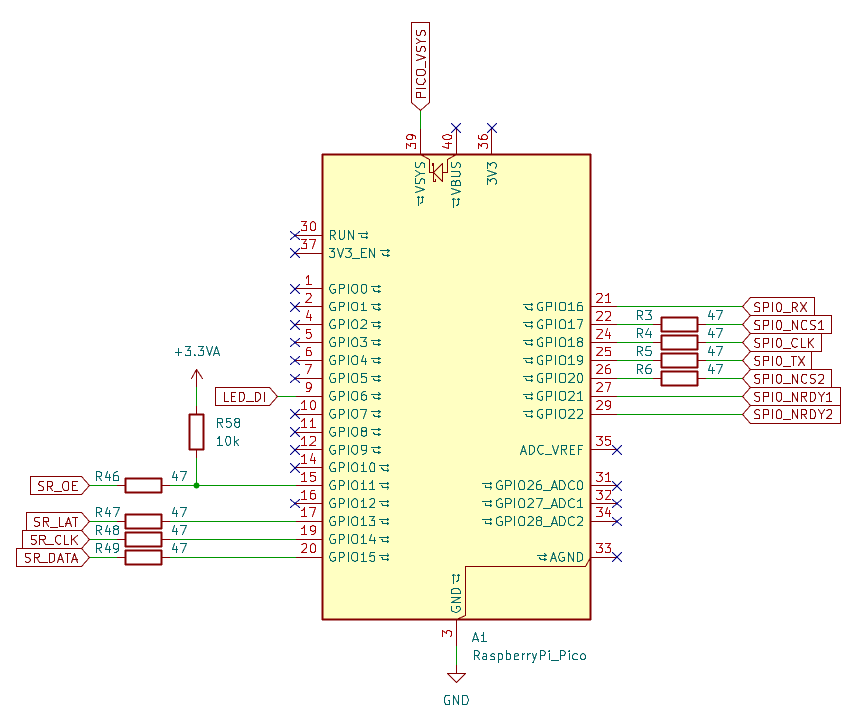
\includegraphics[width=0.75\linewidth]{04-implementation/figures/microcontroller}
  \titledcaption{Microcontroller}{\scaffoldinline{Name the two SPI buses, the \qty{47}{\ohm} series resistors R3--R6 and R46--R49, the LED data line and the unconnected supply pins. Source: KiCad sheet \code{hardware/Microcontroller.kicad\_sch}.}}
  \label{fig:microcontroller}
\end{figure}

\scaffold{
  \textbf{Paragraph 2, power input.} Walk through the left part of \cref{fig:power-supply}: barrel jack, resettable fuse MF-MSMF050-2 against overcurrent, bidirectional TVS diode SMBJ15CA against voltage spikes, and the P-channel MOSFET DMP3099L as reverse-polarity protection, its gate pulled to ground through \qty{100}{\kilo\ohm} and clamped by a \qty{15}{\volt} Zener diode. Give the reason for each part in a subordinate clause.
}

\scaffold{
  \textbf{Paragraph 3, rails.} Three ADP7142 LDOs \cite{adi2025adp7142} supply \qty{5}{\volt} (LEDs, level shifter and the Pico's VSYS through a Schottky diode that prevents back-feeding when the Pico's USB is connected), \qty{3.3}{\volt} (ADCs, shift registers, switches) and \qty{2.5}{\volt}. The \qty{2.5}{\volt} rail is cascaded from the \qty{3.3}{\volt} rail rather than from the input, so the reference sits behind two regulators. Solder jumpers JP1--JP3 between each LDO and its rail allow the current of every rail to be measured separately. One consequence for operation: the measurement rails derive only from the barrel jack, so USB alone powers only the microcontroller.
}

\scaffold{
  \textbf{Paragraph 4, LED power budget.} The \qty{5}{\volt} LDO delivers at most \qty{200}{\milli\ampere} \cite{adi2025adp7142} and is shared by the four LEDs and the Pico; four LEDs at full white would draw about \qty{240}{\milli\ampere}. The LED driver therefore scales every frame to at most 10 of 255 per color channel, about \qty{4}{\percent}, at the lowest driver level, so that no setting can exceed it.
}

\openquestion{LED limit}{
  The final presentation states a limit of about \qty{20}{\percent} (51 of 255); the firmware was later reduced to 10 of 255. Was the reduction made for the power budget, for visual brightness, or because of the WiFi tests? State the final value in the text.
}

\begin{figure}[htbp]
  \centering
  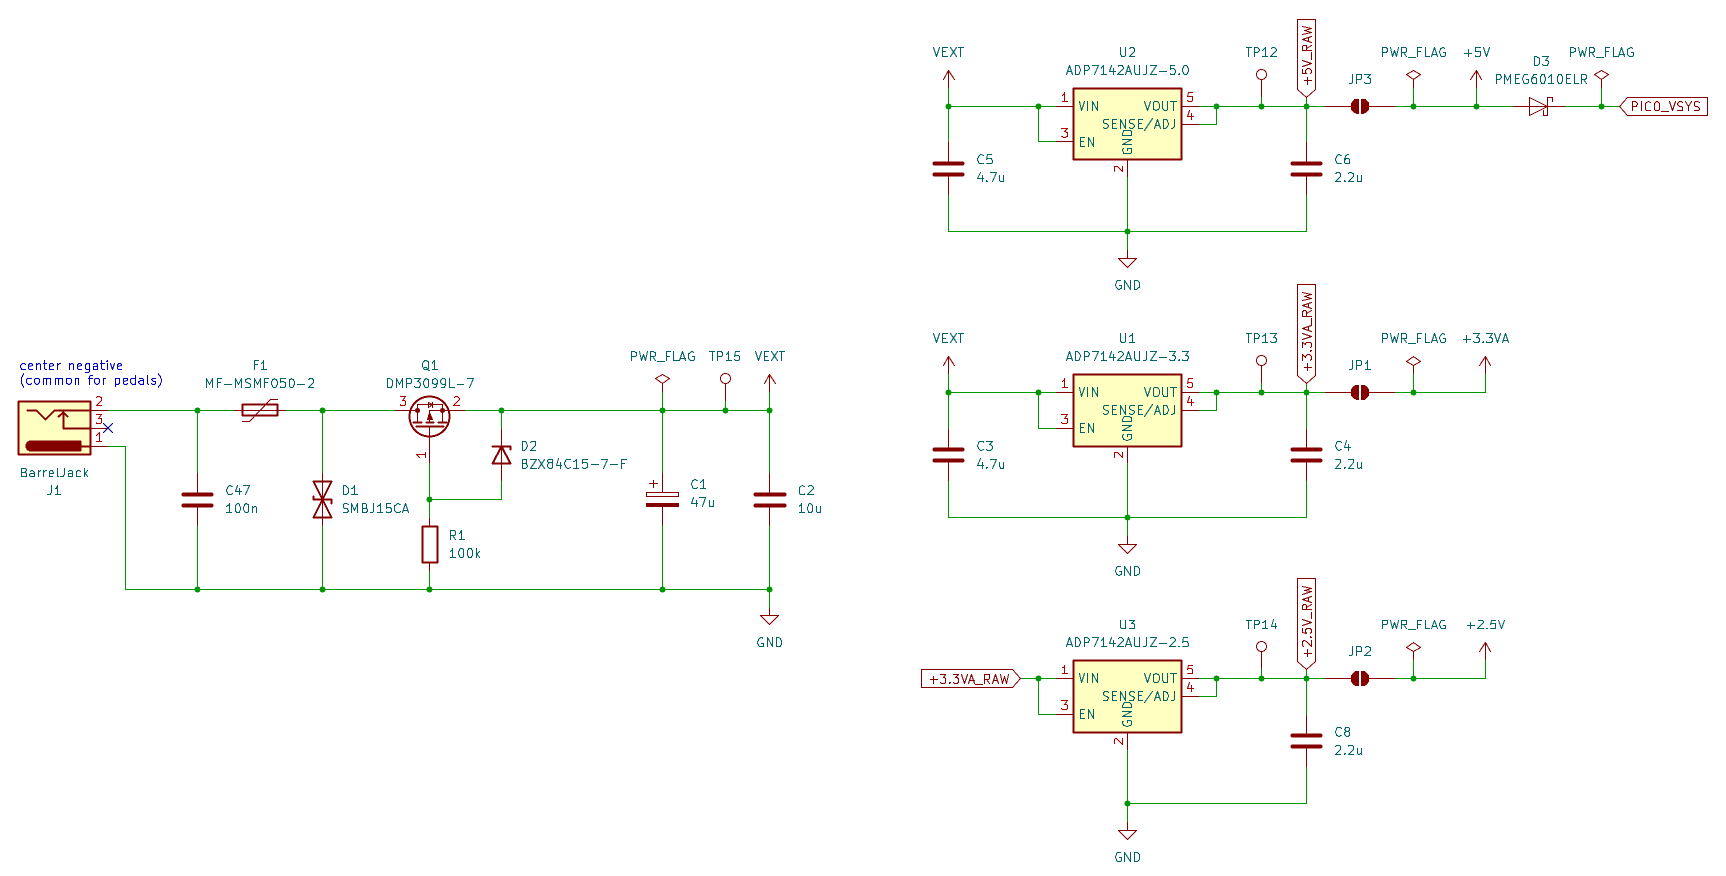
\includegraphics[width=\linewidth]{04-implementation/figures/power-supply}
  \titledcaption{Power Supply}{\scaffoldinline{Name the protection chain (F1, D1, Q1 with R1 and D2), the three LDOs U1--U3 with their output voltages, the cascade of U3 from the \qty{3.3}{\volt} rail, the solder jumpers JP1--JP3 and the Schottky diode D3. Source: KiCad sheet \code{hardware/Power.kicad\_sch}.}}
  \label{fig:power-supply}
\end{figure}
